\refstepcounter{figure}
\noindent Figure \thefigure\ shows throughput variation.

\begin{center}
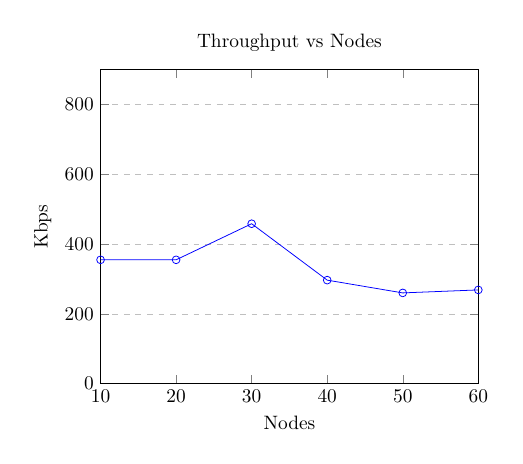
\begin{tikzpicture}[scale=0.7]
\begin{axis}[
title={Throughput vs Nodes},
xlabel={Nodes}, ylabel={Kbps},
xmin=10, xmax=60, ymin=0, ymax=900,
xtick={10,20,30,40,50,60},
ymajorgrids=true, grid style=dashed,
]

\addplot[color=blue, mark=o] coordinates {(10,355.06) (20,355.06) (30,458.57) (40,296.79) (50,260.18) (60,268.75)};

\end{axis}
\end{tikzpicture}

\textbf{Figure \thefigure: Throughput vs Nodes}
\label{fig:throughput_density}
\end{center}